\documentclass[a4j]{jarticle}
    \usepackage[dvipdfmx]{graphicx}
    \usepackage[ top=25truemm,bottom=25truemm,left=25truemm,right=25truemm]
    {geometry}
    \usepackage{ascmac}
    \usepackage{amsmath}
    \usepackage{array}
    \usepackage{here}
    \usepackage{url}
    \usepackage{listings, jlisting}
    \usepackage{cases}
    \usepackage{color}
    \usepackage[subrefformat=parens]{subcaption}
    \renewcommand{\lstlistingname}{リスト}
    \def\vector#1{\mbox{\boldmath $#1$}}
\lstset{language=c,
  basicstyle=\ttfamily\scriptsize,
  commentstyle=\textit,
  classoffset=1,
  keywordstyle=\bfseries,
  frame=tRBl,
  framesep=5pt,
  showstringspaces=false,
  numbers=left,
  stepnumber=1,
  numberstyle=\tiny,
  tabsize=4
}

\makeatletter
\def\@thesis{シミュレーション レポート}
\def\id#1{\def\@id{#1}}
\def\department#1{\def\@department{#1}}

\def\@maketitle{
\begin{center}
{\huge \@thesis \par} %修士論文と記載される部分
\vspace{10mm}
{\LARGE\bf \@title \par}% 論文のタイトル部分
\vspace{10mm}
{\Large \@date\par}	% 提出年月日部分
\vspace{20mm}
{\Large \@department \par}	% 所属部分
{\Large 学籍番号 \@id \par}	% 学籍番号部分
\vspace{10mm}
{\Large 氏名 \@author}% 氏名 
\end{center}
\par\vskip 1.5em
}

\title{第6回~第10回}
\date{提出日 2021年7月15日 1~2コマ目}
\department{組番号 408}
\id{17406}
\author{金澤雄大}

    \begin{document}
    \maketitle
    \thispagestyle{empty}
    \clearpage
    \addtocounter{page}{-1}

    \textcolor{red}{\Huge コピペをさせるためにGitHubにソースやpdfを公開しているわけではありません.公開している理由はみんなとソースコードや実行結果を共有してお互いにより良いものを作りたいからです.
    人のレポ―トをコピペや,体裁をそのままに内容を変えて提出するのはやめましょう.} \clearpage
    \section{目的}

    \section{実験環境}
      実験環境を表\ref{env}に示す.gccはWindows上のWSL(Windows Subsystem for Linux)で動作するものを用いる.
      \begin{table}[H]
        \caption{実験環境}
      \label{env}
      \begin{center}
          \begin{tabular}{c|l}\hline
            CPU & AMD Ryzen 5 3600 6-Core Processor \\ 
            メモリ & 16.0GB DDR4 \\
            OS & Microsoft Windows 10 Home \\
            gcc & (Ubuntu 9.3.0-17ubuntu1~20.04) 9.3.0 \\
            Make & GNU Make 4.2.1 \\ \hline
          \end{tabular}
      \end{center}
      \end{table}

      \section{課題6}
      本章では課題6における課題内容,プログラムの説明,実行結果,考察の4つについて述べる.
      \subsection{課題内容}
      式(\ref{rotoka})の方程式はロトカ・ヴォルテラの方程式と呼ばれる微分方程式である.ロトカ・ヴォルテラの方程式は2種類の生物の個体数の変化に関する数理モデルである.
      式(\ref{rotoka})は被食者(食べられる側)の個体数$y_1$,捕食者(食べる側)の個体数$y_2$としたときの個体数の変化を表している
      .本課題では式(\ref{rotoka})をオイラー法で実装し,正の実数定数$a$,$b$,$c$,$d$を変化させたときの解の特徴について考察する.
      \begin{eqnarray}
      \begin{cases}
        \frac{dy_1}{dx} = ay_1-cy_1y_2 & \\
        \frac{dy_2}{dx} = -by_2+dy_1y_2 &
      \end{cases}
      \label{rotoka}
    \end{eqnarray}

      \subsection{プログラムの説明}
      本節では実装のための理論および次に示す6つの関数の機能,およびソースコードについて説明する.
      \begin{enumerate}
        \item multipleMatrix関数
        \item addVector関数
        \item scalerVector関数
        \item transformVector関数
        \item setVector関数
        \item main関数
      \end{enumerate}

      \subsubsection{実装のための理論}
      本項では,はじめに2変数の単純な連立微分方程式について考え,一般変数に理論を拡張する.
      はじめに2変数の単純な連立方程式について考える.式(\ref{linear_case})の微分方程式をオイラー法で
      解く方法を考える.ただし,$a$に添え字がついているものはすべて定数である.注目してほしいのは右辺で,$y_1$,$y_2$の一次式になっていることがわかる.

      \begin{eqnarray}
      \begin{cases}
        \frac{dy_1}{dx} = a_{11} + a_{12} y_1 + a_{13} y_2 & \\
        \frac{dy_2}{dx} = a_{21} + a_{22} y_1 + a_{23} y_2 &
      \end{cases}
      \label{linear_case}
    \end{eqnarray}      

     オイラー法を用いると式(\ref{linear_case})は時間$t+1$のとき式(\ref{linear_case_euler})のように近似できる.
    ただし,$h$は刻み幅とする.
    \begin{eqnarray}
      \begin{cases}
        y_1(t+1) = y_1(t) + h(a_{11} + a_{12} y_1(t) + a_{13} y_2(t)) & \\
        y_2(t+1) = y_2(t) + h(a_{21} + a_{22} y_1(t) + a_{23} y_2(t)) &
      \end{cases}
      \label{linear_case_euler}
    \end{eqnarray}      
    
    式(\ref{linear_case_euler})を実装すれば2変数の場合には問題なく実行できる.しかし,これを3変数,4変数と拡張しようとすると
    C言語では不都合が生じる.例えば式(\ref{linear_case})の右辺を関数として実装した場合,
    変数が増えるごとに関数の数が増えてしまい拡張性やメンテナンス性が悪い.このため式(\ref{linear_case_euler})では一般変数に対応できない.
    そこで行列を用いる.式(\ref{linear_case_euler})を行列を用いて表すと式(\ref{linear_case_mat})のようになる.
    \begin{eqnarray}
        \left(
          \begin{array}{c}
            y_1(t+1)  \\
            y_2(t+1)  
          \end{array}
        \right)
      =
        \left(
          \begin{array}{ccc}
            y_1(t) \\
            y_2(t) 
          \end{array}
        \right)
        +
        h\left(
          \begin{array}{ccc}
            a_{11} & a_{12} & a_{13} \\
            a_{21} & a_{22} & a_{23}
          \end{array}
        \right)
        \left(
          \begin{array}{ccc}
            1 \\
            y_1(t) \\
            y_2(t)
          \end{array}
        \right)
      \label{linear_case_mat}
    \end{eqnarray}

     式(\ref{linear_case_mat})を参考にして,一般に$y_1$,$y_2$...$y_n$のn個の連立微分方程式(式\ref{linear_case_n})があるとき,
    オイラー法による数値解は式(\ref{linear_case_mat_n})の行列を用いることで計算できる.本課題では式(\ref{linear_case_mat_n})を実装する.
    \begin{eqnarray}
      \begin{cases}
        \frac{dy_1}{dx} = a_{11} + a_{12} y_1 + a_{13} y_2 + \cdots + a_{1n+1} y_n & \\
        \frac{dy_2}{dx} = a_{21} + a_{22} y_1 + a_{23} y_2 + \cdots + a_{2n+1} y_n & \\
             \vdots & \\
        \frac{dy_n}{dx} = a_{n1} + a_{n2} y_1 + a_{n3} y_2 + \cdots + a_{nn+1} y_n
      \end{cases}
      \label{linear_case_n}
    \end{eqnarray}      

    \begin{eqnarray}
      \left(
        \begin{array}{c}
          y_1(t+1)  \\
          y_2(t+1)  \\
          \vdots \\
          y_n(t+1) 
        \end{array}
      \right)
    =
    \left(
      \begin{array}{c}
        y_1(t)  \\
        y_2(t)  \\
        \vdots \\
        y_n(t) 
      \end{array}
    \right)
      +
      h\left(
        \begin{array}{cccc}
          a_{11} & a_{12} & \cdots & a_{1n+1} \\
          a_{21} & a_{22} & \cdots & a_{2n+1} \\
          \vdots & \vdots & \ddots & \vdots \\
          a_{n1} & a_{n2} & \cdots & a_{nn+1}
        \end{array}
      \right)
      \left(
        \begin{array}{c}
          1 \\
          y_1(t) \\
          y_2(t) \\
          \vdots \\
          y_n(t)
        \end{array}
      \right)
    \label{linear_case_mat_n}
  \end{eqnarray}

   式(\ref{rotoka})のロトカ・ヴォルテラの方程式は$y_1y_2$という相互作用項を含んでいるが,式(\ref{linear_case_mat_n})の
  行列によるオイラー法の数値計算はこれに対応していない.式(\ref{rotoka})の方程式を行列で表すと式(\ref{rotoka_mat})のようになる.
  これによって相互作用項を対応させることができる.式(\ref{rotoka_mat})から,行列の積,ベクトルの変換,ベクトルのスカラー倍,ベクトルの和の4つの
  演算が必要であることがわかる.
  しかし,式(\ref{rotoka_mat})では$y_1(t+1)\cdot y_2(t+1) =  y_1y_2(t+1)$が成立していないため,$y_1(t)y_2(t)$を$y_1(t)\cdot y_2(t)$に置き換える必要がある.
  \begin{eqnarray}
    \left(
      \begin{array}{c}
        y_1(t+1)  \\
        y_2(t+1)  \\
        y_1y_2(t+1) 
      \end{array}
    \right)
  =
    \left(
      \begin{array}{ccc}
        y_1(t) \\
        y_2(t) \\
        y_1y_2(t)
      \end{array}
    \right)
    +
    h\left(
      \begin{array}{cccc}
        0 & a & 0 & -c \\
        0 & 0 & -b & d \\
        0 & 0 & 0 & 0
      \end{array}
    \right)
    \left(
      \begin{array}{ccc}
        1 \\
        y_1(t) \\
        y_2(t) \\
        y_1y_2(t)
      \end{array}
    \right)
  \label{rotoka_mat}
\end{eqnarray}

      \subsubsection{multipleMatrix関数}
      multipleMatrix関数は行列の積を計算する関数である.表\ref{multipleMatrixtable}にmultipleMatrix関数の機能,引数,返り値の3つを示す.
      multipleMatrix関数は$n \times (n+1)$行列と$(n+1) \times 1$行列の積を計算する機能を持つから,引数としてa,b,cの3つの行列をとる設計になっている.
      そして引数a,bの行列積abをcに代入する処理を行う.ただし,DIMはオブジェクト形式マクロで定義されている微分方程式の変数の数である.
      \begin{table}[H]
        \caption{multipleMatrix関数の機能,引数,返り値}
        \label{multipleMatrixtable}
        \begin{center}
            \begin{tabular}{c|l}\hline
          機能 & $n \times (n+1)$行列と$(n+1) \times 1$行列の行列積を計算する\\
          引数 & double a[DIM][DIM+1],double b[DIM+1][1],double c[DIM][1] \\
          返り値 & なし\\ \hline
            \end{tabular}
        \end{center}
        \end{table}

        リスト\ref{multipleMatrix}にmultipleMatrix関数のソースコードを示す.リスト\ref{multipleMatrix}では
        引数の行列a,bの積をfor文を用いて計算し,その結果を引数cに代入する処理を行っている.
    \begin{lstlisting}[basicstyle=\ttfamily\footnotesize, frame=single,label=multipleMatrix,caption=multipleMatrix関数のコード]
#define DIM 3

void multipleMatrix(double a[DIM][DIM+1],double b[DIM+1][1],double c[DIM][1]){
    int i,j,k;
    double tmp;
    tmp=0;
      for(i=0; i<DIM+1; i++){
        for(j=0; j<DIM; j++){
            c[i][j]=0;
            for(k=0; k<DIM+1; k++){
	            c[i][j]+=a[i][k]*b[k][j];
      }
    }
  }
}
    \end{lstlisting}

      \subsubsection{addVector関数}
      addVector関数はベクトルの和を計算する関数である.表\ref{addVectortable}にaddVector関数の機能,引数,返り値の3つを示す.
      addVector関数は2つの$n$次元ベクトルの和を計算する機能を持つから,引数としてa,b,cの3つのベクトルをとる設計になっている.
      そして,引数a,bの和を計算し,cに代入する処理を行う.
        \begin{table}[H]
          \caption{addVector関数の機能,引数,返り値}
          \label{addVectortable}
          \begin{center}
              \begin{tabular}{c|l}\hline
                機能 & 2つの$n$次元ベクトルの和を計算する\\
                引数 & double a[DIM][1],double b[DIM][1],double c[DIM][1] \\
                返り値 & なし\\ \hline
              \end{tabular}
          \end{center}
          \end{table}

          リスト\ref{addVector}にaddVector関数のソースコードを示す.リスト\ref{addVector}では
        引数a,bの和をfor文を用いて計算し,その結果を引数cに代入する処理を行っている.
    \begin{lstlisting}[basicstyle=\ttfamily\footnotesize, frame=single,label=addVector,caption=addVector関数のコード]
void addVector(double a[DIM][1],double b[DIM][1],double c[DIM][1]){
    int i;
    for(i=0; i<DIM;i++){
        c[i][0] = a[i][0]+b[i][0];
    }
}
    \end{lstlisting}

      \subsubsection{scalerVector関数}
      scalerVector関数はベクトルのスカラー倍を計算する関数である.表\ref{scalerVectortable}にscalerVector関数の機能,引数,返り値の3つを示す.
      scalerVector関数はベクトルのスカラー倍を計算する機能を持つから,引数としてベクトルa,スカラーhをとる設計になっている.
      そして,引数aのh倍を計算し,aを更新する処理を行う.
        \begin{table}[H]
          \caption{scalerVector関数の機能,引数,返り値}
          \label{scalerVectortable}
          \begin{center}
              \begin{tabular}{c|l}\hline
                機能 & ベクトルのスカラー倍を計算する\\
                引数 & double a[DIM][1],double h \\
                返り値 & なし\\ \hline
              \end{tabular}
          \end{center}
          \end{table}

          リスト\ref{scalerVector}にscalerVector関数のソースコードを示す.リスト\ref{scalerVector}では
        引数aのh倍をfor文を用いて計算し,その結果をaに代入する処理を行っている.
    \begin{lstlisting}[basicstyle=\ttfamily\footnotesize, frame=single,label=scalerVector,caption=scalerVector関数のコード]
void scalerVector(double a[DIM][1],double h){
    int i;
    for(i=0; i<DIM;i++){
        a[i][0] *=h;
    }
}
    \end{lstlisting}

      \subsubsection{transformVector関数}
      transformVector関数は$n$次元ベクトル$\vector{x}=(x_1,x_2,\dots,x_n)$を$(n+1)$次元ベクトル
      $\vector{x}'=(1,x_1,x_2,\dots,x_n)$に変換する関数である.
      表\ref{transformVectortable}にtransformVector関数の機能,引数,返り値の3つを示す.
      transformVector関数はベクトル変換をする機能を持つから,引数として$n$次元ベクトルaおよび$(n+1)$次元ベクトルb
      をとる設計になっている.そして,引数aの変換を計算し,bに代入する処理を行う.
        \begin{table}[H]
          \caption{transformVector関数の機能,引数,返り値}
          \label{transformVectortable}
          \begin{center}
              \begin{tabular}{c|l}\hline
                機能 & ベクトルの変換を行う\\
                引数 & double a[DIM][1],double b[DIM+1][1] \\
                返り値 & なし\\ \hline
              \end{tabular}
          \end{center}
          \end{table}

          リスト\ref{transformVector}にtransformVector関数のソースコードを示す.リスト\ref{transformVector}では
        b[0][0]に1を代入し,他のb成分には引数aの成分をfor文を用いて代入する処理を行っている.
    \begin{lstlisting}[basicstyle=\ttfamily\footnotesize, frame=single,label=transformVector,caption=transformVector関数のコード]
void transformVector(double a[DIM][1],double b[DIM+1][1]){
    int i;
    b[0][0]=1;
    for(i=1; i<DIM+1;i++){
        b[i][0] = a[i-1][0];
    }
}
    \end{lstlisting}

      \subsubsection{setVector関数}
      setVector関数はベクトルの値を別の変数に代入する関数である.表\ref{setVectortable}にsetVector関数の機能,引数,返り値の3つを示す.
      setVector関数はベクトルの値を別の変数に代入する機能を持つから,引数としてベクトルa,bをとる設計になっている.
      そして,引数aを引数bに代入する処理を行う.
        \begin{table}[H]
          \caption{setVector関数の機能,引数,返り値}
          \label{setVectortable}
          \begin{center}
              \begin{tabular}{c|l}\hline
                機能 & ベクトルの値を別の変数に代入する\\
                引数 & double a[DIM][1],double b[DIM][1]\\
                返り値 & なし\\ \hline
              \end{tabular}
          \end{center}
          \end{table}

          リスト\ref{setVector}にsetVector関数のソースコードを示す.リスト\ref{setVector}では
        引数aをfor文を用いてbに代入する処理を行っている.
    \begin{lstlisting}[basicstyle=\ttfamily\footnotesize, frame=single,label=setVector,caption=setVector関数のコード]
void setVector(double a[DIM][1],double b[DIM][1]){
    int i;
    for(i=0;i<DIM;i++){
        b[i][0] = a[i][0];
    }
}
    \end{lstlisting}


      \subsubsection{main関数}
      main関数はEuler法を用いて連立微分方程式を計算する.表\ref{maintable}にmain関数の機能,引数,返り値の3つを示す.
      main関数は
        \begin{table}[H]
          \caption{main関数の機能,引数,返り値}
          \label{maintable}
          \begin{center}
              \begin{tabular}{c|l}\hline
                機能 & 連立微分方程式の計算を行う\\
                引数 & なし(void)\\
                返り値 & (int)0\\ \hline
              \end{tabular}
          \end{center}
          \end{table}

          リスト\ref{main1}にmain関数のソースコードを示す.
    \begin{lstlisting}[basicstyle=\ttfamily\footnotesize, frame=single,label=main1,caption=main関数のコード]
int main(void){
    double h = 0.1;
    double lim=1.01;
    double a=0.7;
    double b=0.4;
    double c=0.09;
    double d=0.06;
    double y10=10;
    double y20=10;
    double step;
    int i;

    // 初期値を宣言するベクトルの配列
    double initVector[DIM][1] ={{y10},{y20},{y10*y20}};
    // ベクトル変換用配列
    double transVector[DIM+1][1];
    // 連立微分方程式のパラメータの配列
    double weightMatrix[DIM][DIM+1] = {{0,a,0,-c},
                                       {0,0,-b,d},
                                       {0,0,0,0}
                                       };
    // 計算用配列
    double yiVector[DIM][1];
    double tmpVector[DIM][1];
    //結果表示用配列
    double resultVector[DIM][1];

    // 初期値表示
    #ifdef STDOUT
    printf("step = %0.2lf\n",0.1);
    #else
    printf("%lf,%lf,%lf",0.0,initVector[0][0],initVector[1][0]);
    #endif

        for(i=0;i<DIM;i++){
            #ifdef STDOUT
            printf("y%d = %lf\n",i,initVector[i][0]);
            #endif
        }
        printf("\n");

    // 初期値を計算用配列にセット
    setVector(initVector,yiVector);

    for(step=h;step<=lim;step+=h){
        //ベクトル変換
        transformVector(yiVector,transVector);
        // 微分係数を計算
        multipleMatrix(weightMatrix,transVector,tmpVector);
        scalerVector(tmpVector,h);
        // 1次ラグとの和を計算
        addVector(yiVector,tmpVector,resultVector);

        //結果を表示
        #ifdef STROUT
        printf("step = %0.2lf\n",step);
        for(i=0;i<DIM;i++){
            printf("y%d = %lf\n",i,resultVector[i][0]);
        }
        printf("\n");
        #else
        printf("%lf,%lf,%lf\n",step,resultVector[0][0],resultVector[1][0]);
        #endif

        // y1*y2調整処理
        resultVector[2][0] = resultVector[0][0]*resultVector[1][0];
        // 結果を計算用配列にセット
        setVector(resultVector,yiVector);
    }
    return 0;
}
\end{lstlisting}
リスト\ref{main1}では次に示す手順で処理を行っている.
\begin{enumerate}
  \item ステップ数,連立方程式のパラメータの値,初期条件の値,ループ用変数の4つを宣言する(リスト\ref{main1}の2行目から11行目).
  \item 初期条件をinitVectorという変数で宣言する(リスト\ref{main1}の14行目).
  \item ベクトル変換用の配列をtransVectorという変数で宣言する(リスト\ref{main1}の16行目).
  \item 連立方程式のパラメータをweightMatrixという変数で宣言する(リスト\ref{main1}の18行目).
  \item 計算および結果表示用の配列を宣言する(リスト\ref{main1}の23行目から26行目).
  \item 初期値を表示する.本プログラムでは条件付きコンパイルを用いる.オブジェクト形式マクロでSTDOUTが宣言されているときは
  標準出力に適したフォーマットで計算結果を出力する.CSVOUTが定義されているときは,csv出力に適したフォーマットで出力する
  (リスト\ref{main1}の29行目から40行目).
  \item 計算用配列に初期条件をセットする(リスト\ref{main1}の43行目).
  \item ステップ数に応じて手順9から手順14を反復実行する.
  \item ベクトルの変換を行う.ここでの変換とは$n$次元ベクトル$\vector{x}=(x_1,x_2,\dots,x_n)$を$(n+1)$次元ベクトル
  $\vector{x}'=(1,x_1,x_2,\dots,x_n)$にする変換のことである(リスト\ref{main1}の47行目).
  \item 行列の積を用いて微分係数を計算する(リスト\ref{main1}の49行目から50行目).
  \item ベクトルの和を用いてEuler法の近似計算を行う(リスト\ref{main1}の52行目).
  \item 結果を表示する.表示形式は手順6と同様にSTDOUT,CSVOUTの場合分けが行われている(リスト\ref{main1}の55行目から63行目).
  \item $y_1(t)y_2(t)$の調整を行う(リスト\ref{main1}の66行目).
  \item 次のステップの計算のために計算結果を計算用配列にセットする(リスト\ref{main1}の68行目).
\end{enumerate}

      \subsection{実行結果}
      実行結果は連立微分方程式のパラメータ$a$,$b$,$c$,$d$の値によって異なると考えられる.パラメータ$a$,$b$,$c$,$d$の大小
      で実験結果が異なると仮定すると,実験が必要なパラメータの組み合わせは,表\ref{result1-plan}のようになる.
      本節では実験1から実験4までの実行結果について述べる.
      \begin{table}[H]
        \caption{実験計画}
      \label{result1-plan}
      \begin{center}
          \begin{tabular}{c|c|c}\hline
            条件 & $y_2 > a/c$ & $y_2 < a/c$\\ \hline
            $y_1 > b/d$  & 実験1 & 実験2  \\
            $y_1 < b/d$  & 実験3 & 実験4 \\ \hline
          \end{tabular}
      \end{center}
      \end{table}

       実験1から実験9までのパラメータ$a$,$b$,$c$,$d$を表\ref{result1-params}に示す.
      ただし,$y_1=10,y_2=10$,$h=0.01$は固定とする.実験1および実験4はパラメータを4通りに変化させて実験を行う.実験2および実験3は
      パラメータを2通りに変化させて実験を行う.
      \begin{table}[H]
        \caption{各実験におけるパラメータの設定}
      \label{result1-params}
      \begin{center}
          \begin{tabular}{c|c|c|c|c}\hline
            実験番号 & $a$ & $b$ & $c$ & $d$ \\ \hline \hline
            実験1-1 & 1 & 1 & 1 & 1 \\ \hline
            実験1-2 & 7 & 6 & 1 & 1 \\ \hline
            実験1-3 & 6 & 7 & 0.9 & 0.8 \\ \hline
            実験1-4 & 6 & 7 & 0.8 & 0.9 \\ \hline
            実験2-1 & 3 & 2 & 0.1 & 0.5 \\ \hline
            実験2-2 & 3 & 2 & 0.1 & 0.8 \\ \hline
            実験3-1 & 2 & 3 & 0.5 & 0.1 \\ \hline
            実験3-2 & 2 & 3 & 0.8 & 0.1 \\ \hline
            実験4-1 & 2 & 3 & 0.1 & 0.2 \\ \hline
            実験4-2 & 4 & 5 & 0.3 & 0.4 \\ \hline
            実験4-3 & 3 & 2 & 0.2 & 0.1 \\ \hline
            実験4-4 & 2.1 & 2 & 0.2 & 0.18 \\ \hline
          \end{tabular}
      \end{center}
      \end{table}

      \subsubsection{実験1の結果}
      実験1は,$y_2 > a/c$かつ$y_1 > b/d$の条件下でパラメータを変化させたときの実行結果である.実験1-1から実験1-4
      までの結果を図\ref{exp1}に示す.

        \begin{figure}[H]
          \begin{tabular}{c}
          \begin{minipage}{0.5\hsize}
           \begin{center}
            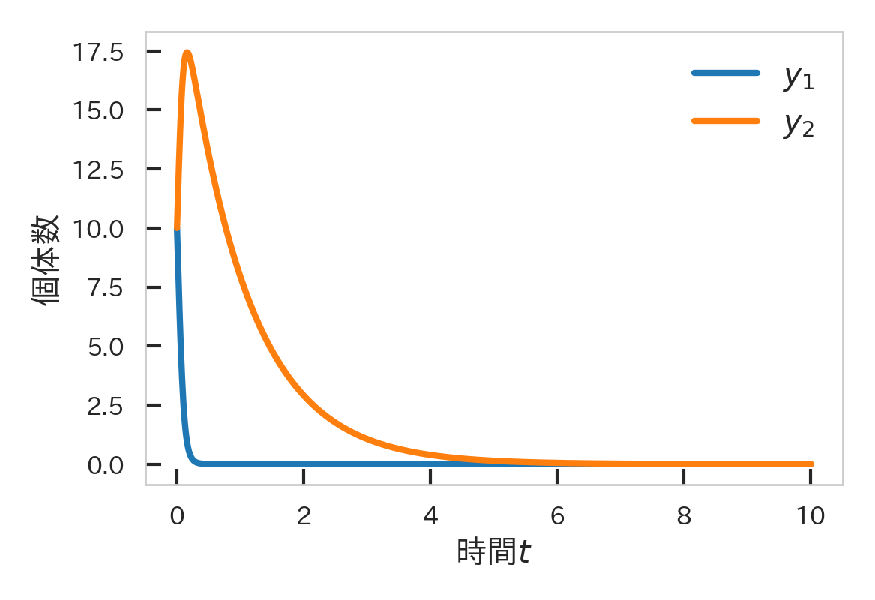
\includegraphics[scale=0.5]{ex1-1.eps}
           \end{center}
           \subcaption{実験1-1}
           \label{ex611}
          \end{minipage}

          \begin{minipage}{0.5\hsize}
           \begin{center}
            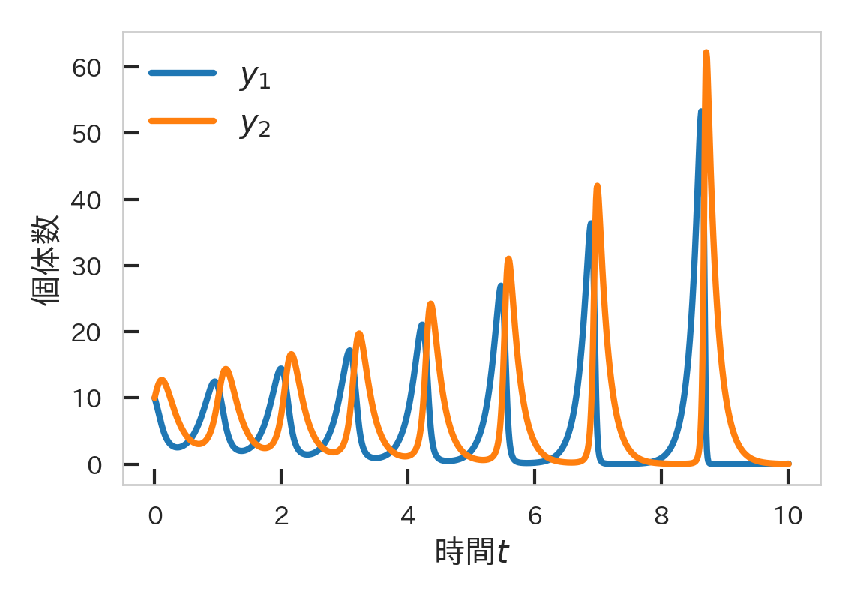
\includegraphics[scale=0.5]{ex1-2.eps}
           \end{center}
           \subcaption{実験1-2}
           \label{ex612}
          \end{minipage}
        \end{tabular}

        \begin{tabular}{c}
          \begin{minipage}{0.5\hsize}
            \begin{center}
             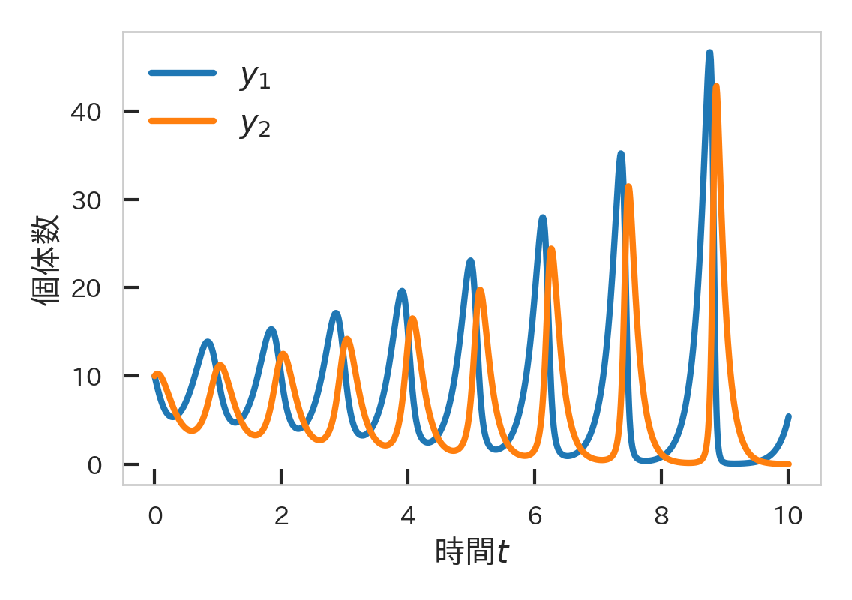
\includegraphics[scale=0.5]{ex1-3.eps}
            \end{center}
            \subcaption{実験1-3}
            \label{ex613}
           \end{minipage}

           \begin{minipage}{0.5\hsize}
            \begin{center}
             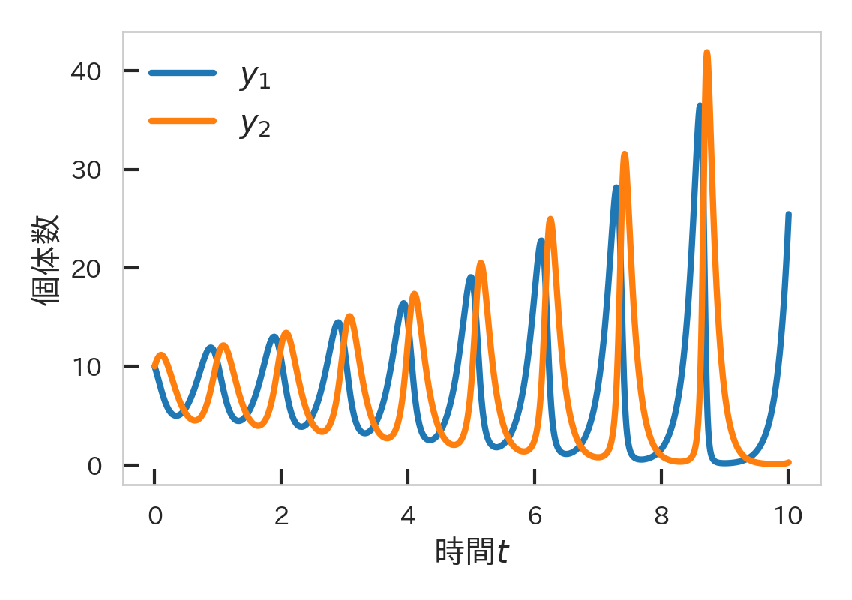
\includegraphics[scale=0.5]{ex1-4.eps}
            \end{center}
            \subcaption{実験1-4}
            \label{ex614}
           \end{minipage}
          \end{tabular}
          \caption{実験1の結果}
          \label{exp1}
         \end{figure}

         図\ref{ex611}は表\ref{result1-params}に示した実験1-1の結果をグラフにしたものである.まず,実行結果と手計算
         で求めたオイラー法の値が一致することを確認する.表\ref{result1-1acc}に実験1-1における実行結果から得られた値と
         手計算によって計算した値である.表\ref{result1-1acc}では時間$t$が0.01から0.03までの場合について,
         手計算行った.
      \begin{table}[H]
        \caption{実験結果と手計算の比較}
      \label{result1-1acc}
      \begin{center}
          \begin{tabular}{c|l l|l l}\hline
             & \multicolumn{2}{c|}{実験結果} & \multicolumn{2}{c}{手計算} \\ \cline{2-5}
             時間$t$ & \multicolumn{1}{c}{$y_1$} & \multicolumn{1}{c|}{$y_2$} & \multicolumn{1}{c}{$y_1$} & \multicolumn{1}{c}{$y_2$} \\ \cline{1-5}
             0 & 10 & 10 & 10 & 10 \\ 
0.01 & 9.1 & 10.9 & 9.1 & 10.9 \\
0.02 & 8.1991 & 11.7829 & 8.1991 & 11.7829 \\
0.03 & 7.314999 & 12.631163 & 7.314999 & 12.631163 \\ \hline
          \end{tabular}
      \end{center}
      \end{table}
      手計算の方法を例を交えて説明する.パラメータはすべて1だから,計算する連立方程式微分方程式は
      式(\ref{all1})である.式(\ref{all1})をオイラー法の計算式にすると式(\ref{all11})になる.
      \begin{eqnarray}
        \begin{cases}
          \frac{dy_1}{dx} = y_1-y_1y_2 & \\
          \frac{dy_2}{dx} = y_2+y_1y_2 &
        \end{cases}
        \label{all1}
      \end{eqnarray}

      \begin{eqnarray}
        \begin{cases}
          y_{1(i+1)} = y_{1(i)}+h(y_{1(i)} + y_{1(i)}y_{2(i)}) & \\
          y_{2(i+1)} = y_{2(i)}+h(-y_{2(i)} + y_{1(i)}y_{2(i)}) &
        \end{cases}
        \label{all11}
      \end{eqnarray}

      $h=0.01$のときの正しい実験結果は,$y_{1(0)}=y_{2(0)}=10$を式(\ref{all11})に代入すると,
      式(\ref{all12})に示すように計算できる.時間を$0.02,0.03 \dots $と変化させた場合も
      同じように計算を行えばよい.
      \begin{eqnarray}
        \begin{cases}
          y_{1(0.01)} = 10+0.01\cdot (10 + 10\cdot 10) = 9.1& \\
          y_{2(0.01)} = 10+0.01\cdot (-10 + 10\cdot 10) = 10.9&
        \end{cases}
        \label{all12}
      \end{eqnarray}
       表\ref{result1-1acc}の実験結果と手計算の結果から,時間$t$が$0.01$から$0.03$のとき,
      実行結果と手計算の結果が一致していることがわかる.時間$t$が$0.01$から$0.03$の3例で
      すべての実行結果と手計算に誤差がないとは言えないから,excelによる計算結果と実行結果
      を比較する.図\ref{gosa}にexcelによる計算と実行結果の差を示す.
      \begin{figure}[H]
        \centering
        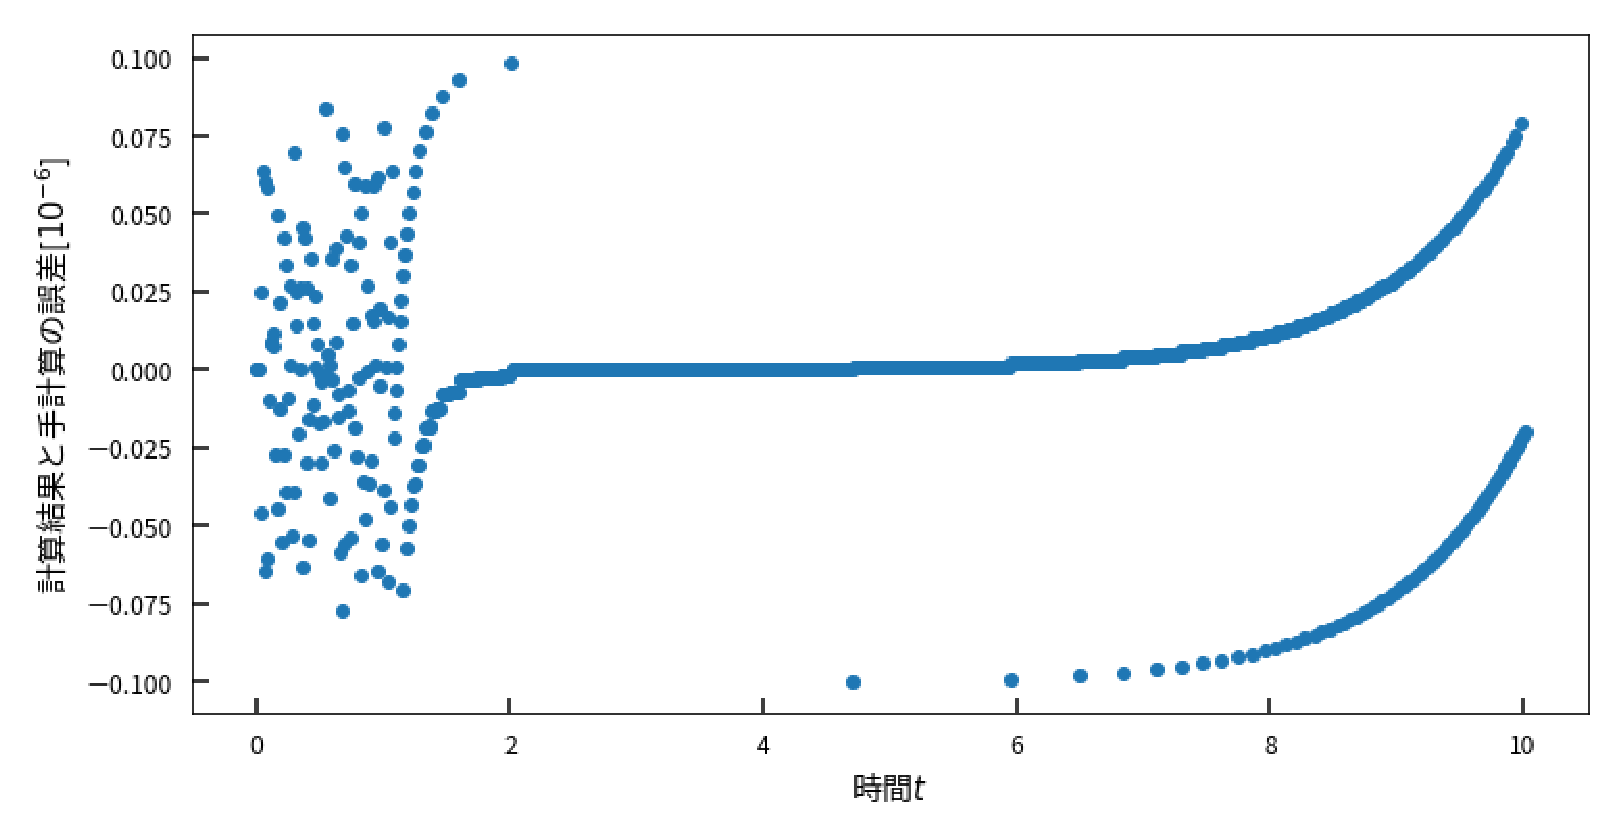
\includegraphics[scale=0.5]{ex11error.eps}
        \caption{計算結果の差}
         \label{gosa}
        \end{figure}
        
        図\ref{gosa}において,手計算と実行結果の差は$10^{-7}$程度であることがわかる.
        これより,実行結果と手計算が一致していると考えられる.よって実行結果は正しいと
        言える.\\
         実行結果が正しいことがわかったから,パラメータを変化させたときの実行結果
        について観察する.実験1の4つの実験結果に共通していることは,$y_1$,$y_2$の値
        が0以上であるということである.$y_1$は被食者,$y_2$は捕食者を表していた.
        式(\ref{rotoka})のモデルの特性は後で考察するが,$y_1$,$y_2$が
        非負であることは,モデルによる生物の個体数の増減のシミュレーションの
        結果が非常にわかりやすくなる.さらに,$a$,$b$を固定して,$c$,$d$を入れ替えた
        実験1-3,実験1-4の結果に注目する.実験1-3と実験1-4の結果は$y_1$,$y_2$が入れ替わ
        っただけである.このことから,$a$,$b$を固定したとき,$c$,$d$は対称関係にあり,
        $c$,$d$のうち,値の大きいほうが,周期的な立ち上がりが大きいことがわかる.
      

      \subsubsection{実験2の結果}
      実験2は,$y_2 < a/c$かつ$y_1 > b/d$の条件下でパラメータを変化させたときの実行結果である.実験2-1および実験2-2
      結果を図\ref{exp2}に示す.図\ref{exp2}から,実験2の条件では被食者$y_2$が周期的に大量発生し,捕食者$y_1$は20前後の
      数字であることが読み取れる.このことから,$y_2 < a/c$という条件が満たされるようなモデルは,被食者が周期的に
      大量発生し,捕食者は被食者と比較すると少数であることが考えられる.

      \begin{figure}[H]
        \begin{tabular}{c}
        \begin{minipage}{0.5\hsize}
         \begin{center}
          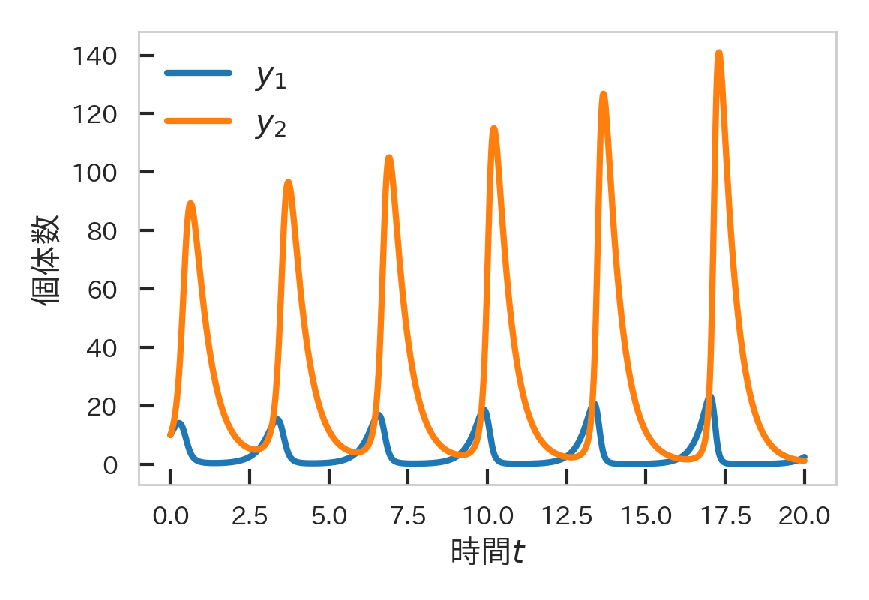
\includegraphics[scale=0.5]{ex2-1.eps}
         \end{center}
         \subcaption{実験2-1}
         \label{ex621}
        \end{minipage}

        \begin{minipage}{0.5\hsize}
         \begin{center}
          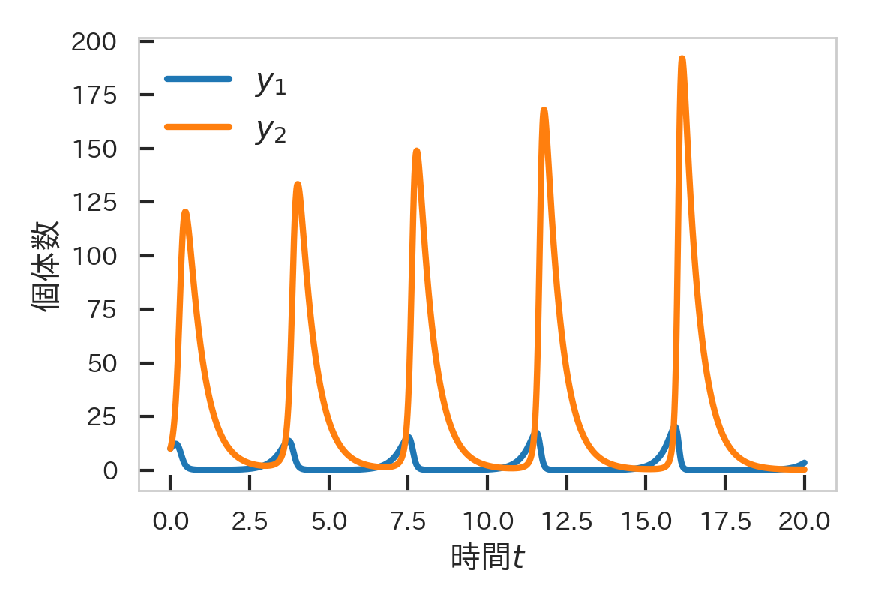
\includegraphics[scale=0.5]{ex2-2.eps}
         \end{center}
         \subcaption{実験2-2}
         \label{ex622}
        \end{minipage}
      \end{tabular}
        \caption{実験2の結果}
        \label{exp2}
       \end{figure}

      \subsubsection{実験3の結果}
      実験3は,$y_2 > a/c$かつ$y_1 < b/d$の条件下でパラメータを変化させたときの実行結果である.実験3-1および実験3-2
      結果を図\ref{exp3}に示す.図\ref{exp3}から,実験3の条件では実験2とは逆に,被食者$y_1$が周期的に大量発生し,
      捕食者$y_2$は少数であることが読み取れる.実験2および実験3から,$y_2 > a/c$または$y_1 > b/d$というどちらかの
      条件を満たすモデルでは,被食者と捕食者のバランスが悪いシミュレーション結果が得られることが考えられる.さらに,
      実験2,実験3のどちらにおいても,個体数が0に限りなく近づくタイミングがあることがわかる.今扱っているモデルでは
      連続なモデルを考えているから,個体数が0に限りなく近づいても上昇することがあるが,実際には生態系のバランス崩れた
      ことで絶滅したと考えることもできる.

      \begin{figure}[H]
        \begin{tabular}{c}
        \begin{minipage}{0.5\hsize}
         \begin{center}
          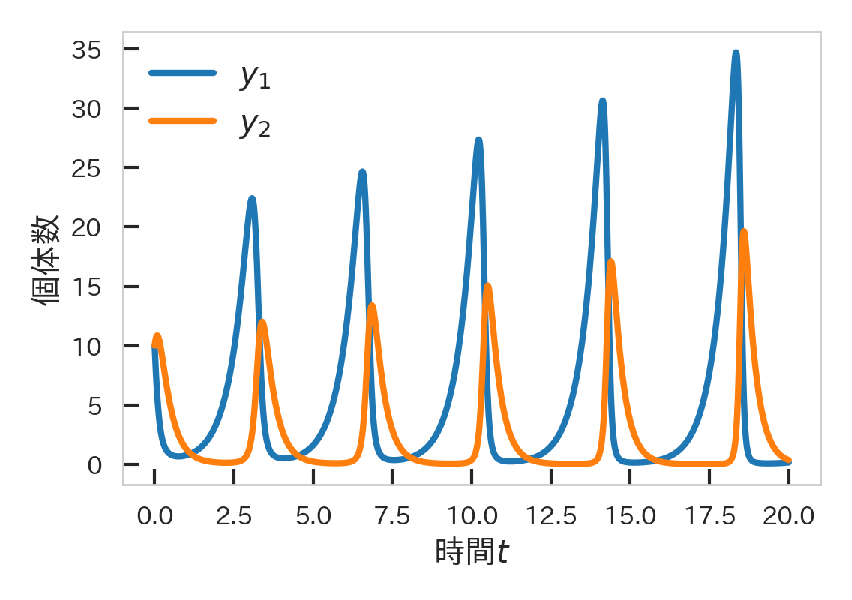
\includegraphics[scale=0.5]{ex3-1.eps}
         \end{center}
         \subcaption{実験3-1}
         \label{ex631}
        \end{minipage}

        \begin{minipage}{0.5\hsize}
         \begin{center}
          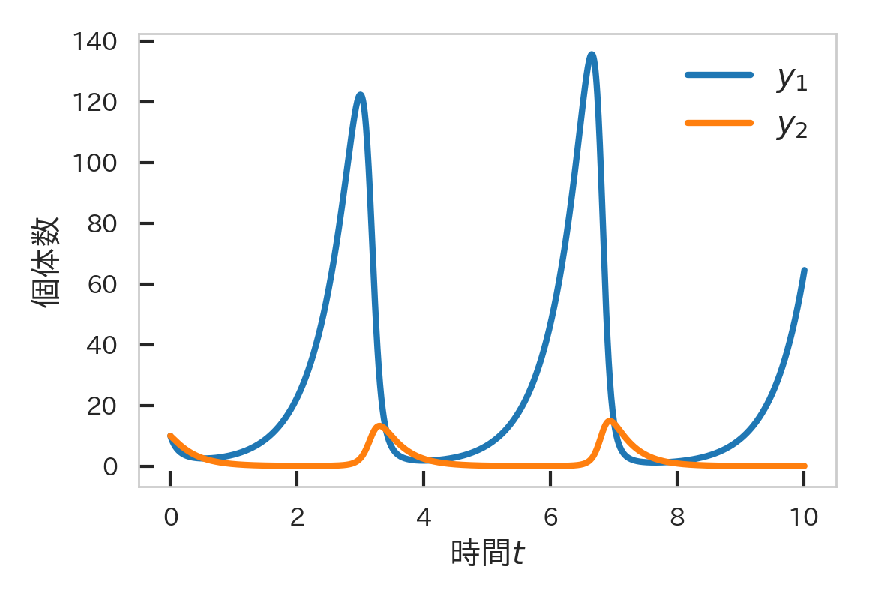
\includegraphics[scale=0.5]{ex3-2.eps}
         \end{center}
         \subcaption{実験3-2}
         \label{ex632}
        \end{minipage}
      \end{tabular}
        \caption{実験3の結果}
        \label{exp3}
       \end{figure}

      \subsubsection{実験4の結果}
      実験4は,$y_2 < a/c$かつ$y_1 < b/d$の条件下でパラメータを変化させたときの実行結果である.実験4-1から実験4-2
      までの結果を図\ref{exp4}に示す.図\ref{exp4}から実験4の結果は,パラメータによってまったく違うことが読み取れる.
      図\ref{ex641}は$y_1$,$y_2$ともに個体数が安定しており,個体数が0,つまり絶滅しにくいモデルであることが読み取れる.
      図\ref{ex642}は個体の周期的な増減に加えて,全体にトレンドがあるように見える.図\ref{ex643}は$y_1$,$y_2$の周期的な
      増加のピークの値が,増加しているモデルであるように見える.図\ref{ex644}は$t=2$で$y_1$,$y_2$ともに絶滅するモデルで
      あると読み取れる.

      \begin{figure}[H]
        \begin{tabular}{c}
        \begin{minipage}{0.5\hsize}
         \begin{center}
          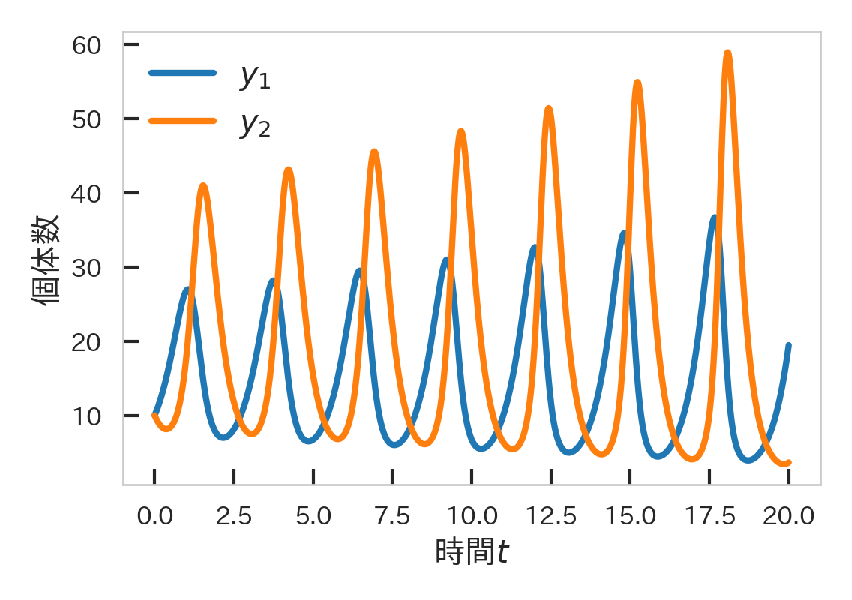
\includegraphics[scale=0.5]{ex4-1.eps}
         \end{center}
         \subcaption{実験4-1}
         \label{ex641}
        \end{minipage}

        \begin{minipage}{0.5\hsize}
         \begin{center}
          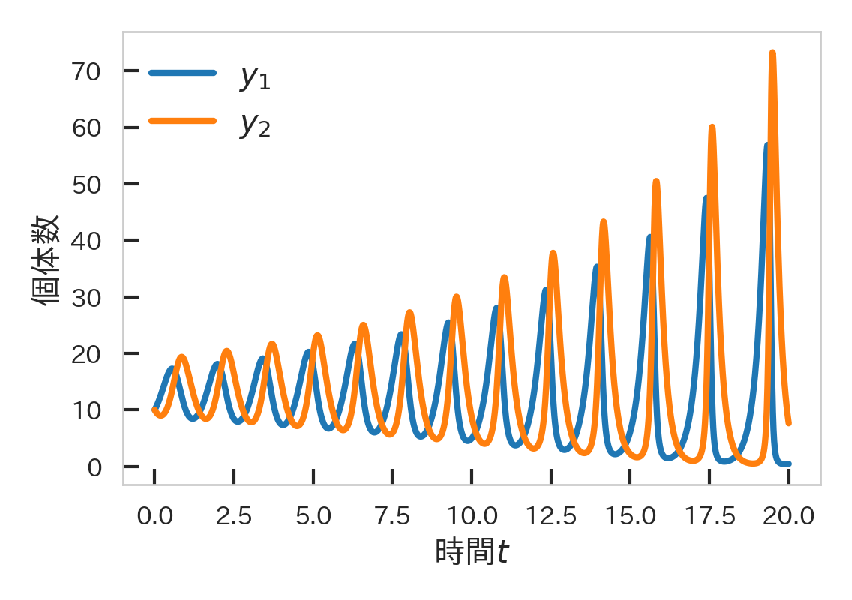
\includegraphics[scale=0.5]{ex4-2.eps}
         \end{center}
         \subcaption{実験4-2}
         \label{ex642}
        \end{minipage}
      \end{tabular}

      \begin{tabular}{c}
        \begin{minipage}{0.5\hsize}
          \begin{center}
           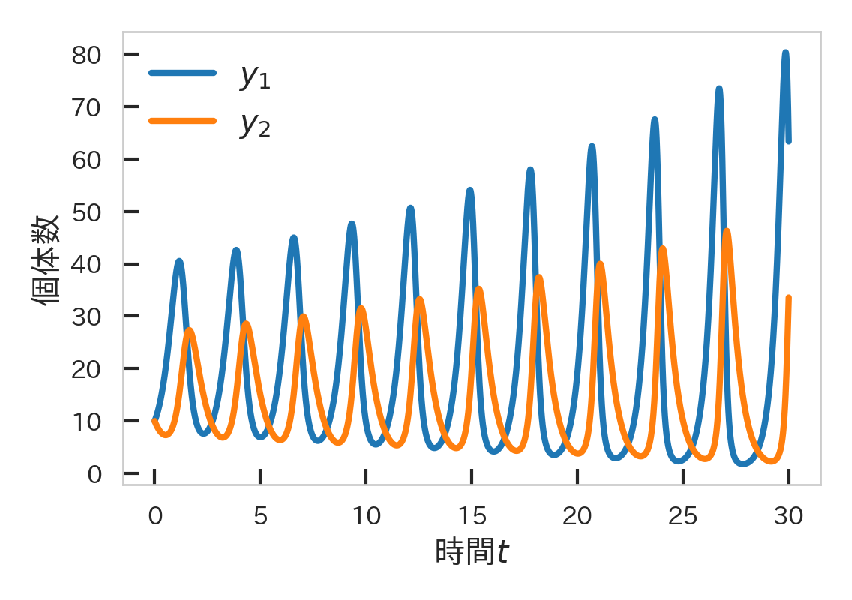
\includegraphics[scale=0.5]{ex4-3.eps}
          \end{center}
          \subcaption{実験4-3}
          \label{ex643}
         \end{minipage}

         \begin{minipage}{0.5\hsize}
          \begin{center}
           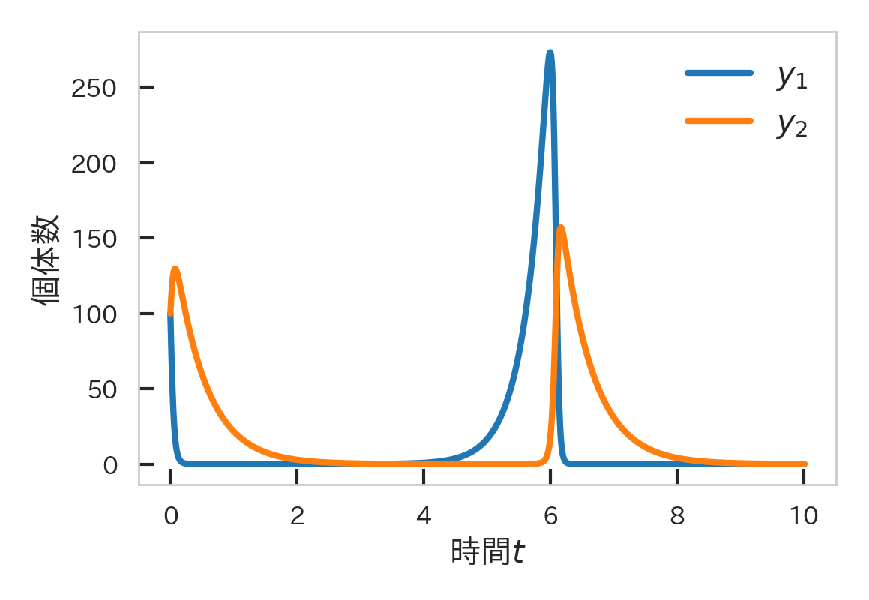
\includegraphics[scale=0.5]{ex4-4.eps}
          \end{center}
          \subcaption{実験4-4}
          \label{ex644}
         \end{minipage}
        \end{tabular}
        \caption{実験4の結果}
        \label{exp4}
       \end{figure}

      \subsection{考察}
       実験1~4の結果から,パラメータa,b,c,dの意味を考察する.式(\ref{rotoka})からパラメータaは
       被食者の繁殖のしやすさ,パラメータbは捕食者の減少のしやすさを意味すると考えられる.パラメータcは
       実験2から捕食者の数に比例した被食者の減少のしやすさであると考えられる.パラメータdは実験3から
       被食者の数に比例した捕食者の繁殖のしやすさであると考える.
       

      \section{課題7}
      本章では課題7における,課題内容,プログラムの説明,実行結果の3つについて述べる.
      \subsection{課題内容}
      質量$m$の物体がばね定数$k$のばねにくっついているときの単振動のシミュレーションを行う.
      この運動方程式は式(\ref{soe})のように書ける.高階微分方程式をそのまま数値計算を行うことは
      できない.我々が扱えるのは,連立微分方程式であるから,これに帰着するように式変形を行う.
      \begin{equation}
        \frac{d^2x}{dt^2}+\frac{k}{m}x=0
        \label{soe}
      \end{equation}
      $v=\frac{dx}{dt}$とおくと,式(\ref{soe})は式(\ref{bane})で表せる.式(\ref{bane})は
      連立方程式微分方程式であるから,課題6のプログラムを改変すれば数値計算を行うことができる.
      \begin{eqnarray}
        \begin{cases}
          v = \frac{dx}{dt} & \\
          \frac{dv}{dt} = -kx &
        \end{cases}
        \label{bane}
      \end{eqnarray}


      \subsection{プログラムの説明}
      課題7のプログラムは,課題6のプログラムのメイン関数を改変しただけである.リスト\ref{main7}にメイン関数のコードを示す.

      \begin{lstlisting}[basicstyle=\ttfamily\footnotesize, frame=single,label=main7,caption=メイン関数のコード]
int main(void){
    double h = 0.01;
    double lim=10.0;
    double m=1;
    double k=2;
    double l=0;
    double step;
    int i;
    double initVector[DIM][1] ={{10},{0}}; // 初期条件 y,v 
    double transVector[DIM+1][1];
    double weightMatrix[DIM][DIM+1] = {{0,0,1},
                                        {0,-k/m,-l/m}
                                       };
    double yiVector[DIM][1];
    double tmpVector[DIM][1];
    double resultVector[DIM][1];

    setVector(initVector,yiVector);
    for(step=h;step<=lim;step+=h){
        transformVector(yiVector,transVector);
        multipleMatrix(weightMatrix,transVector,tmpVector);
        scalerVector(tmpVector,h);
        addVector(yiVector,tmpVector,resultVector);
        /* format for stdout
        printf("step = %0.2lf\n",step);
        printf("y = %lf\n",resultVector[0][0]);
        printf("v = %lf\n",resultVector[1][0]);
        printf("\n");
        */
        printf("%0.2lf,%lf,%lf\n",step,resultVector[0][0],resultVector[1][0]);

        setVector(resultVector,yiVector);
    }
    return 0;
}
            \end{lstlisting}     
      \subsection{実行結果}
      
      \subsection{考察}
      \section{課題8}
      本章では課題8における,課題内容,プログラムの説明,実行結果の3つについて述べる.
      \subsection{課題内容}
      \subsection{プログラムの説明}
      \subsection{実行結果}
      \section{課題9}
      本章では課題9における,課題内容,プログラムの説明,実行結果の3つについて述べる.
      \subsection{課題内容}
      \subsection{プログラムの説明}
      \subsection{実行結果}
      \subsection{考察}
      \section{課題10}
      本章では課題10における,課題内容,プログラムの説明,実行結果の3つについて述べる.
      \subsection{課題内容}
      \subsection{プログラムの説明}
      \subsection{実行結果}
      \subsection{考察}

        \begin{thebibliography}{9}
          \bibitem{NNCT}  国立高専機構長野高専,\url{http://www.nagano-nct.ac.jp/} ,閲覧日2020年8月5日
          \end{thebibliography}
\end{document}

